%% osm-intro.tex
%%


\section{Introduction}

\frame { \heading{OSM: kesako?} \vfill

  OpenStreetMap (OSM) est un \textbf{projet collaboratif} visant à créer des
  \textbf{cartes libres}

  \begin{itemize}
  \item données et cartes rediffusables sous licence libre 
\includegraphics[width=1.2cm]{figures/cc-by-sa}
  \item couvrant toute la planète
  \item modèle de contribution à la wiki: chacun peut ajouter des
    traces GPS, corriger le nom d'une rue
  \item projet fondé en 2004, croissance très rapide
  \end{itemize}

  \vfil
  
\begin{beamerboxesrounded}[width=\textwidth,scheme=alert,shadow=true]{} \sffamily\footnotesize
  «OpenStreetMap is a project aimed squarely at creating and
  providing free geographic data such as street maps to anyone who
  wants them. The project was started because most maps you think of
  as free actually have legal or technical restrictions on their use,
  holding back people from using them in creative, productive or
  unexpected ways.»
\end{beamerboxesrounded}

}


%% animation Toulouse timeline



\frame{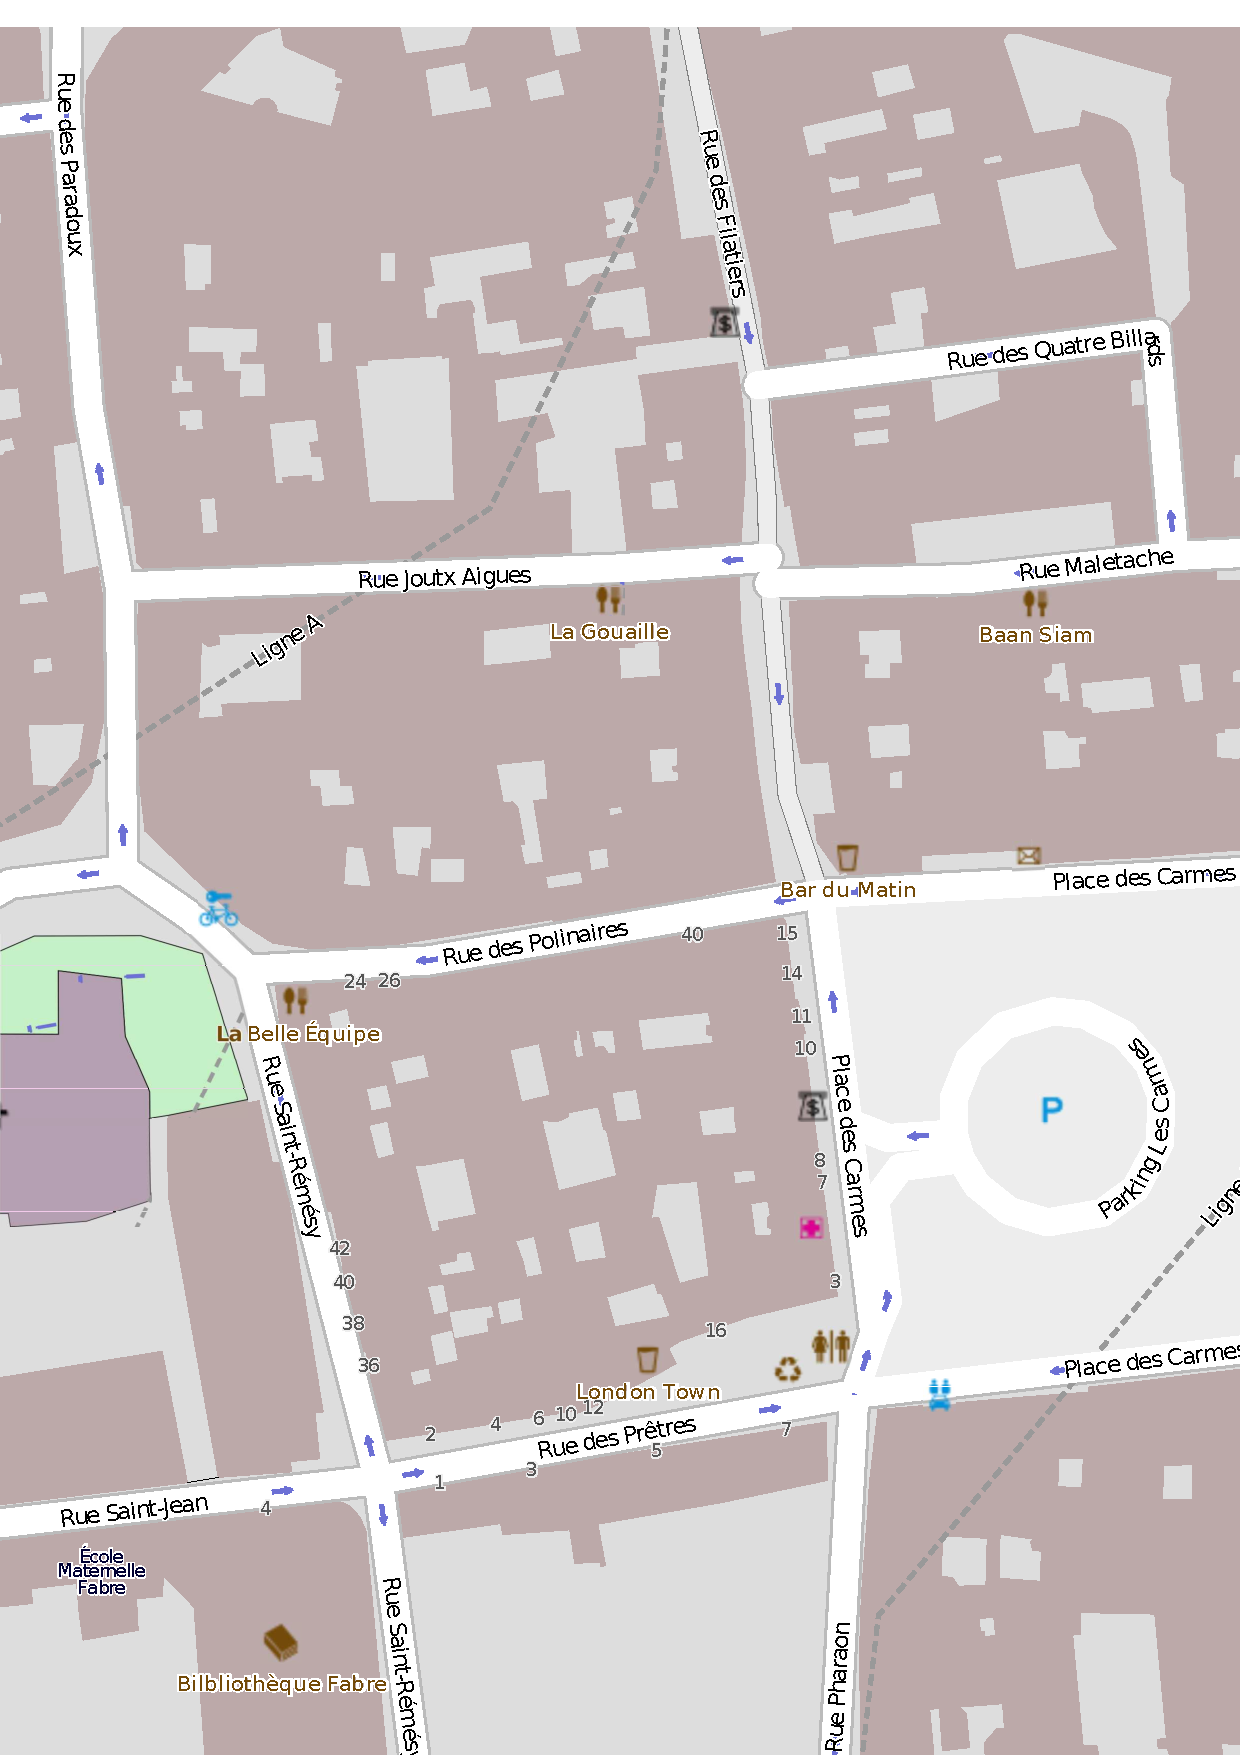
\includegraphics[width=0.95\textwidth,clip,trim=0cm 2cm 0cm 4cm]{figures/toulouse-carmes}}

% \frame{\includegraphics[width=0.95\textwidth]{figures/toulouse-zoom}}



\frame{
  %% http://www.flickr.com/photos/stevefaeembra/3674760067/sizes/o/in/set-72157620624558941/
 \hskip-0.5cm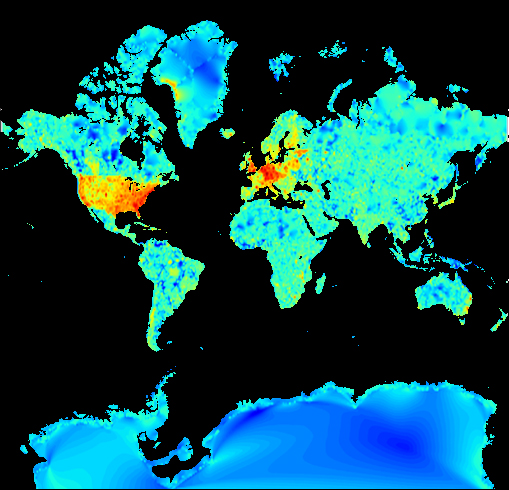
\includegraphics[width=0.8\textwidth]{figures/osm-heatmap}

 %% http://www.openstreetmap.org/stats/data_stats.html

 {\small Décembre 2009}
 
\begin{tikzpicture}[remember picture,overlay,font={\footnotesize},text
    width=2cm,text centered]
   \node[starburst,fill=yellow,draw=red,line width=2pt,shift={(-2cm,-2cm)}]
      at (current page.north east) {190\,535 utilisateurs};
   \node[starburst,fill=yellow,draw=red,line width=2pt,shift={(-3cm,-7.1cm)}]
      at (current page.north east) {1\,300\,501\,165 points GPS};
\end{tikzpicture}
}




\frame{ \heading{Des données libres?} \vfill

  Libertés que devraient offrir des données géographiques:

  \begin{itemize}
  \item utiliser les données dans n'importe quel but
  \item étudier les données et de les adapter
  \item distribuer des copies
  \item modifier les données et rendre publiques ces modifications
  \end{itemize}

\begin{itemize}
% \item[{\color{red}\ding{56}}]
\item[\ecmfrownie] Les principales sources de données aujourd'hui sont non-libres: IGN, INSEE,
  NavTec, Spot Image

\item[\ecmfrownie] Avec Google Maps, je peux calculer un itinéraire pour circuler en
  voiture, mais pas un chemin adapté au vélo.
\end{itemize}
}



%% EOF
